\subsection{Layanan Tiket}

Layanan tiket memproses setiap permintaan yang berkaitan dengan pemesanan tiket. Layanan ini dapat dipecah menjadi beberapa layanan bergantung pada desain setiap arsitektur solusi.

\subsubsection{Kebutuhan Fungsional dan Non-Fungsional}

Berikut adalah kebutuhan fungsional layanan tiket:

\begingroup
\footnotesize
\begin{longtable}{|l|p{0.4\textwidth}|p{0.4\textwidth}|}
    \caption{Kebutuhan Fungsional Layanan Tiket}                                                                                                                                                                                                                                                                                                                                                                                                                                                                                                                                                           \\
    \hline
    \textbf{ID} & \textbf{Kebutuhan}                                                                                                                                                                                                              & \textbf{Deskripsi}                                                                                                                                                                                                                                                                                                                                    \\
    \endfirsthead

    \multicolumn{3}{|l|}{\tablename\ \thetable\ -- \textit{Lanjutan dari halaman sebelumnya}}                                                                                                                                                                                                                                                                                                                                                                                                                                                                                                             \\
    \hline
    \textbf{ID} & \textbf{Kebutuhan}                                                                                                                                                                                                              & \textbf{Deskripsi}                                                                                                                                                                                                                                                                                                                                    \\
    \endhead

    \hline
    \multicolumn{3}{|r|}{\textit{Dilanjutkan ke halaman berikutnya}}                                                                                                                                                                                                                                                                                                                                                                                                                                                                                                                                      \\
    \endfoot

    \hline
    \endlastfoot

    \hline
    TF-01       & Sistem dapat melayani permintaan ketersediaan acara.                                                                                                                                                                            &                                                                                                                                                                                                                                                                                                                                                       \\
    \hline
    TF-02       & Sistem dapat melayani permintaan ketersediaan tiket untuk suatu acara .                                                                                                                                                         & Ketersediaan tiket dibagi berdasarkan kategori. Data ketersediaan bisa lebih granular (menampilkan ketersediaan per kursi) atau hanya menampilkan jumlah ketersediaan untuk suatu kategori. Perilaku ini dapat diatur per kategori tiket.                                                                                                             \\
    \hline
    TF-03       & Sistem dapat melayani permintaan pemesanan tiket untuk suatu acara. Sebuah acara dapat dilaksanakan selama beberapa hari pada tempat yang sama dengan setiap tiket hanya berlaku pada hari itu saja. & Seorang pengguna dapat memesan hingga lima tiket dalam kategori yang sama sekaligus. Pengguna dapat memesan berdasarkan kursi atau area tiket, bergantung pada pengaturan kategori tiket. Pemesanan akan dibatalkan secara otomatis ketika sudah melewati tenggat waktu pembayaran.                                                                   \\
    \hline
    TF-04       & Pengguna dapat melihat status tiket yang pernah dipesan.                                                                                                                                                                        &                                                                                                                                                                                                                                                                                                                                                       \\
    \hline
    TF-05       & Sistem dapat menangani penjualan tiket untuk lebih dari satu acara dalam satu waktu.                                                                                                                                            &                                                                                                                                                                                                                                                                                                                                                       \\

\end{longtable}
\endgroup

Berikut adalah kebutuhan non-fungsional layanan tiket:

\begingroup
\footnotesize
\begin{longtable}{|l|p{0.4\textwidth}|p{0.5\textwidth}|}
    \caption{Kebutuhan Non-Fungsional Sistem Tiket}                                                                                                                                                                            \\
    \hline
    \textbf{ID} & \textbf{Parameter}                   & \textbf{Kebutuhan}                                                                                                                                                    \\    \endfirsthead

    \multicolumn{3}{|l|}{\tablename\ \thetable\ -- \textit{Lanjutan dari halaman sebelumnya}}                                                                                                                                  \\
    \hline
    \textbf{ID} & \textbf{Parameter}                   & \textbf{Kebutuhan}                                                                                                                                                    \\
    \endhead

    \hline
    \multicolumn{3}{|r|}{\textit{Dilanjutkan ke halaman berikutnya}}                                                                                                                                                           \\
    \endfoot

    \hline
    \endlastfoot

    \hline
    TN-01       & Konsistensi dan integritas transaksi & Sistem harus memastikan tidak terjadi pemesanan ganda pada saat pemesanan tiket.                                                                              \\
    \hline
    TN-02       & Keterbaruan Data              & Sistem harus selalu mengembalikan data ketersediaan paling terbaru.                                                                                                                \\
\end{longtable}
\endgroup

\pagebreak

\subsubsection{Entitas Layanan}

Berikut adalah gambaran diagram relasi entitas pada layanan tiket:

\begin{figure}[htbp]
    \centering
    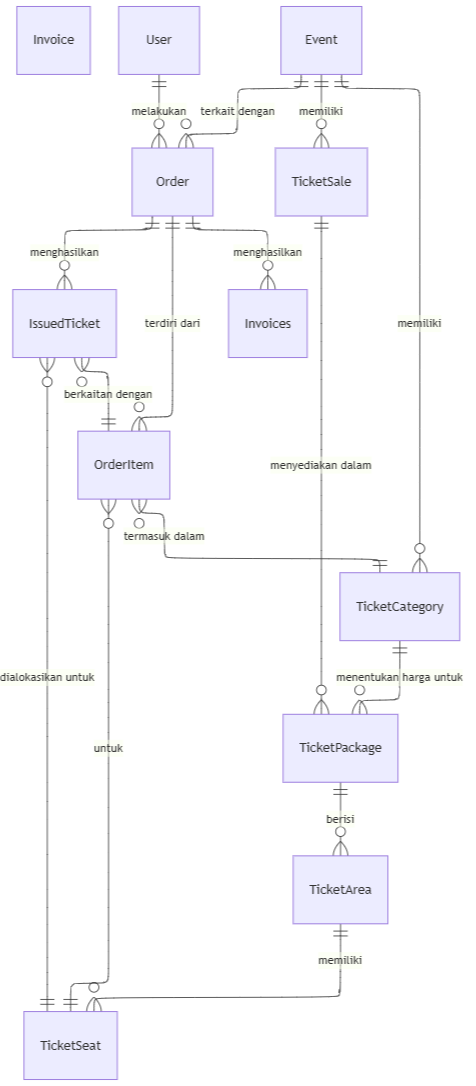
\includegraphics[width=0.5\textwidth]{resources/chapter-3/erd-mini.png}
    \caption{ERD Layanan Tiket}
    \label{fig:erd-ticket-service}
\end{figure}

Skema lengkap setiap entitas dibahas pada bagian lampiran \ref{apx:ticket-schema}. Entitas layanan tiket dapat dibagi menjadi dua grup, yaitu:

\begin{enumerate}
    \item Entitas yang berkaitan dengan tiket dan acara, yaitu: Event, TicketSale, TicketCategory, TicketPackage, TicketArea dan TicketSeat.
    \item Entitas yang berkaitan dengan pemesanan, yaitu: Order, OrderItem, Invoice, dan IssuedTicket.
\end{enumerate}

\pagebreak

Sebuah acara bisa memiliki banyak kategori tiket, seperti tiket kategori reguler, gold, platinum. Setiap kategori tiket bisa meliputi banyak area, seperti tribun timur dan barat. Setiap area terdiri atas banyak Seat dengan status ketersediaan, yaitu tersedia, sedang dipesan, dan terjual.

Entitas TicketSale menunjukkan penjualan tiket yang dilaksanakan pada batas waktu tertentu. Hal ini untuk mengakomodasi penjualan tiket untuk suatu acara yang dilakukan beberapa kali, seperti penjualan tiket \textit{early bird} dan penjualan tiket untuk umum serta untuk mengakomodasi penjualan tiket untuk hari yang berbeda. Setiap TicketSale memiliki banyak TicketPackage yang menandakan kategori tiket yang dijual. Entitas ini terhubung dengan entitas TicketCategory dan memiliki atribut harga. Setiap Seat menunjukkan Seat (fisik) pada hari tertentu. Tiket Seat yang sama pada hari yang berbeda akan memiliki ID yang berbeda. IssuedTicket merupakan tiket yang telah berhasil terjual dan memiliki informasi pemilik tiket dan nomor seri tiket. Untuk menangani penjualan tiket tanpa nomor kursi, sistem membuat penomoran virtual yang akan dipasangkan secara otomatis saat pembelian.

Entitas yang berkaitan dengan pembelian tiket terdiri atas entitas User, Order, OrderItem, dan Invoice. Entitas Invoice ini menyimpan status tagihan yang memiliki berelasi dengan tagihan pada layanan pembayaran. Setiap pesanan terdiri atas banyak OrderItem. Entitas ini menyimpan informasi pemesan dan harga saat pembayaran.

